\documentclass[handout,notes=show]{beamer}
%\documentclass[handout,notes=show]{beamer}
\usepackage{pgfpages}
\pgfpagesuselayout{4 on 1}[letterpaper,landscape, border shrink=5mm]

%\documentclass{beamer}
\usepackage{epstopdf}
\usepackage{amsfonts}
\usepackage{amssymb}
\usepackage{amsmath}

\usepackage{subfig}



\newcommand{\vk}{\ensuremath{\mathbf{k}}}
\newcommand{\vK}{\ensuremath{\mathbf{K}}}
\providecommand{\vr}{\ensuremath{\mathbf{r}}}
%\newcommand{\vec}[1]{\ensuremath{\mathbf{#1}}}

\newcommand{\gk}{\ensuremath{{g}(\mathbf{k})}}

\newcommand{\vp}{\ensuremath{\mathbf{p}}}
\newcommand{\gp}{\ensuremath{{g}(\mathbf{p})}}

\newcommand{\vq}{\ensuremath{\mathbf{q}}}

\newcommand{\Fo}{\ensuremath{\mathbf{F_0}}}


\newcommand{\E}{\ensuremath{\mathbf{E}}}
\newcommand{\A}{\ensuremath{\mathbf{A}}}
\newcommand{\J}{\ensuremath{\mathcal{J}}}

\newcommand{\ket}[1]{\ensuremath{\left|#1\right>}}
\newcommand{\bra}[1]{\ensuremath{\left<#1\right|}}

\newcommand{\twoe}{\ensuremath{2\epsilon_\vk-\E_1}}

\newcommand{\nth}[1]{\ensuremath{\frac{1}{#1}}}

\newcommand{\br}[1]{\ensuremath{\left(#1\right)}}
\newcommand{\mbr}[1]{\ensuremath{\left[#1\right]}}
\newcommand{\bbr}[1]{\ensuremath{\left\{#1\right\}}}


\newcommand{\tk}{\ensuremath{\tilde{k}}}

\newcommand{\kp}{\ensuremath{\ket{\Psi}}}

\newcommand{\av}[1]{\ensuremath{\bigl<{#1}\bigr>}}
\newcommand{\avs}[3] {\av{#1{\lvert{#2}\rvert}#3}}
\newcommand{\avv}[2][\nu] {\avs{#1}{#2}{#1}}
\newcommand{\avt}[2]{\av{{#1}|{#2}}}
\newcommand{\avtu}[1]{\av{T_\tau#1}}

\newcommand{\Bop}{\ensuremath{\mathbf{B_0^+}}}
\newcommand{\Bmp}{\ensuremath{\mathbf{B_m^+}}}
\newcommand{\Bnp}{\ensuremath{\mathbf{B_n^+}}}
\newcommand{\Bo}{\ensuremath{\mathbf{B_0}}}
\newcommand{\Bopn}{\ensuremath{\mathbf{{B_0^+}^n}}}
\newcommand{\Bon}{\ensuremath{\mathbf{{B_0}^n}}}


\newcommand{\zmatrix}{\ensuremath{\br{\begin{smallmatrix}0&0\\0&0\end{smallmatrix}}}}
\newcommand{\fmtrx}[4]{\ensuremath{\br{\begin{smallmatrix}#1&#2\\#3&#4\end{smallmatrix}}}}
\newcommand{\smtrx}[6]{\ensuremath{\br{\begin{smallmatrix}#1&#2\\#3&#4\\#5&#6\end{smallmatrix}}}}

\newcommand{\vz}{\ensuremath{v^{\beta\alpha}_{\vk,\vk}}}


\providecommand{\abs}[1]{\ensuremath{\lvert{#1}\rvert}}

\newcommand{\sg}[1][1]{\ensuremath{\sigma_\frac{#1}{2}}}

\newcommand{\rhof}{\ensuremath{\rho(\ef)}}
\newcommand{\omt}{\ensuremath{\tilde{\Omega}}}
\newcommand{\cht}{\ensuremath{\tilde{\chi_0}}}
\newcommand{\Atl}{\ensuremath{\abs{A}^{2l}}}
\newcommand{\ef}{\ensuremath{\epsilon_F}}

\newcommand{\lca}{\ensuremath{\ln\br{1+\frac{\cht}{\alpha}}}}

\newcommand{\com}[2]{\ensuremath{\mbr{#1,#2}}}
\newcommand{\D}{\ensuremath{\mathit{D}}}
\newcommand{\dg}{\ensuremath{\dagger}}
\newcommand{\nG}{\ensuremath{\hat{\mathcal{G}}^{-1}}}

\providecommand{\lvk}{\ensuremath{1/\vk_F}}
\providecommand{\hm}{\ensuremath{\frac{\hbar^2}}{2m}}
\providecommand{\pdiff}[2]{\ensuremath{\frac{\partial{#1}}{\partial{#2}}}}
\providecommand{\dpdiff}[2]{\ensuremath{\frac{\partial^2{#1}}{\partial{{#2}^2}}}}

\providecommand{\H}{\ensuremath{\mathcal{H}}}
\providecommand{\wt}[1]{\widetilde{#1}}

\providecommand{\eef}[1]{Eq. (\ref{#1})}

\providecommand{\sch}{{Schr\"{o}dinger }}

\providecommand{\sgn}{\ensuremath{\text{sgn}}}
\newcommand{\Arctg}{\ensuremath{\text{Arctg}}}

\providecommand{\comm}[1]{\textit{\scriptsize \uwave{(#1)}}}
\newcommand{\myemph}[1]{\textbf{\color{blue!100}#1}}
\newcommand{\mathemph}[1]{{\color{red}#1}}
% \usepackage{beamerthemesplit} // Activate for custom appearance

\title[Crossover w/ 3-species]{BEC-BCS Crossover with the Feshbach Resonance for a Three-Hyperfine-Species Model}
\author[Guojun Zhu]{Guojun Zhu}
\institute{University of Illinois at Urbana-Champaign}
\date{Dec. 15th, 2011}
\pgfdeclareimage[height=1cm]{university-logo}{uiucLogo2.jpg}
\logo{\pgfuseimage{university-logo}}
%\usetheme[language=english,
%titlepagelogo=logopolito, bullet=circle, pageofpages=of, titleline=true, color=blue
%]{TorinoTh}
%\rel{Anthony J. Leggett}
%\usetheme[hideothersubsections, width=2cm]{PaloAlto}
\usetheme[hideothersubsections]{Berkeley}

%\usetheme{Hannover}
\usecolortheme{sidebartab}
\usefonttheme[onlymath]{serif}
%\usecolortheme{lily}
%\AtBeginSection[]
%{
%  \begin{frame}
%    \frametitle{Table of Contents}
%    \tableofcontents[currentsection]
%  \end{frame}
%}
\begin{document}

\frame{
%\frametitle{Dissertation}
\titlepage}

\section[Outline]{Outline}
\frame{
\frametitle{Outline}
\tableofcontents
}

\section[Atomic Ham.]{Dilute ultracold alkali gas}\label{sec:intro:one}
\frame{

\frametitle{Single-atom Hamiltonian and two-atom interaction}


\begin{itemize}[<+->]
\item Single atom Hamiltonian:
\begin{equation}
H_{spin}=A \mathbf{I}\cdot\mathbf{S}-\mu_{e}\mathbf{B}\cdot\mathbf{S}-{\mu}_{n}\mathbf{B}\cdot\mathbf{I}
\end{equation}
One level splits into a few hyperfine spines, marked by  $(F,F_{z})$.  
$\mathbf{F}=\mathbf{S}+\mathbf{I}$


\item Channels: one  configuration of hyperfine spins for one atom pair in interaction, $\ket{F^{(1)},F_{z}^{(1)}}\otimes\ket{F^{(2)},F_{z}^{(2)}}$ 
\item Interaction mostly due to electrons
\begin{equation}\label{eq:intro:two}
V=f(r)+g(r)\mathbf{S_{1}}\cdot\mathbf{S_{2}}
\end{equation}
\item Short-range potential \& low-energy:  characterized with single parameter, s-wave scattering length, $a_{s}$

\item Channels are mixed.  Resonance are possible. 
\end{itemize}
}



\frame{
 \frametitle{Effective open-channel s-wave scattering length}
\begin{equation}
a_{s}(B)=a_{bg}\br{1+\frac{\Delta{B}}{B-B_{0}}}
\end{equation}
 \begin{figure}[htbp]
\begin{center}
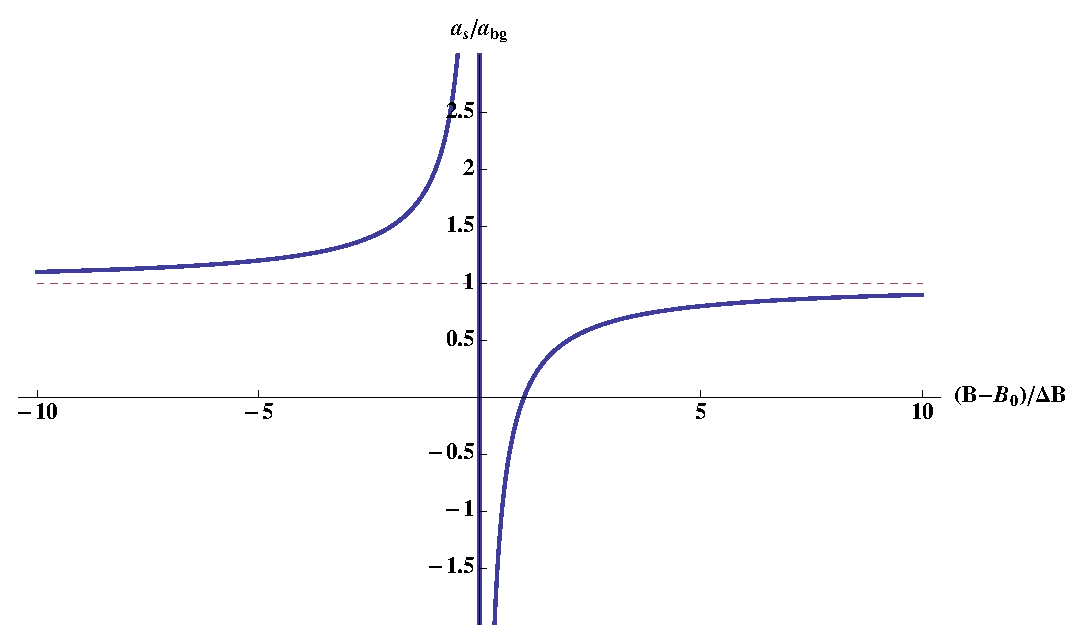
\includegraphics[width=0.8\textwidth]{FeshbachAs}
\caption{S-wave scattering length in Feshbach resonance} 
\label{fig:intro:Feshbach}

\end{center}
\end{figure}

 }
 
 
 \frame{
 \frametitle{Potentials in a Feshbach resonance} 
 
\begin{figure}[htbp]
\begin{center}
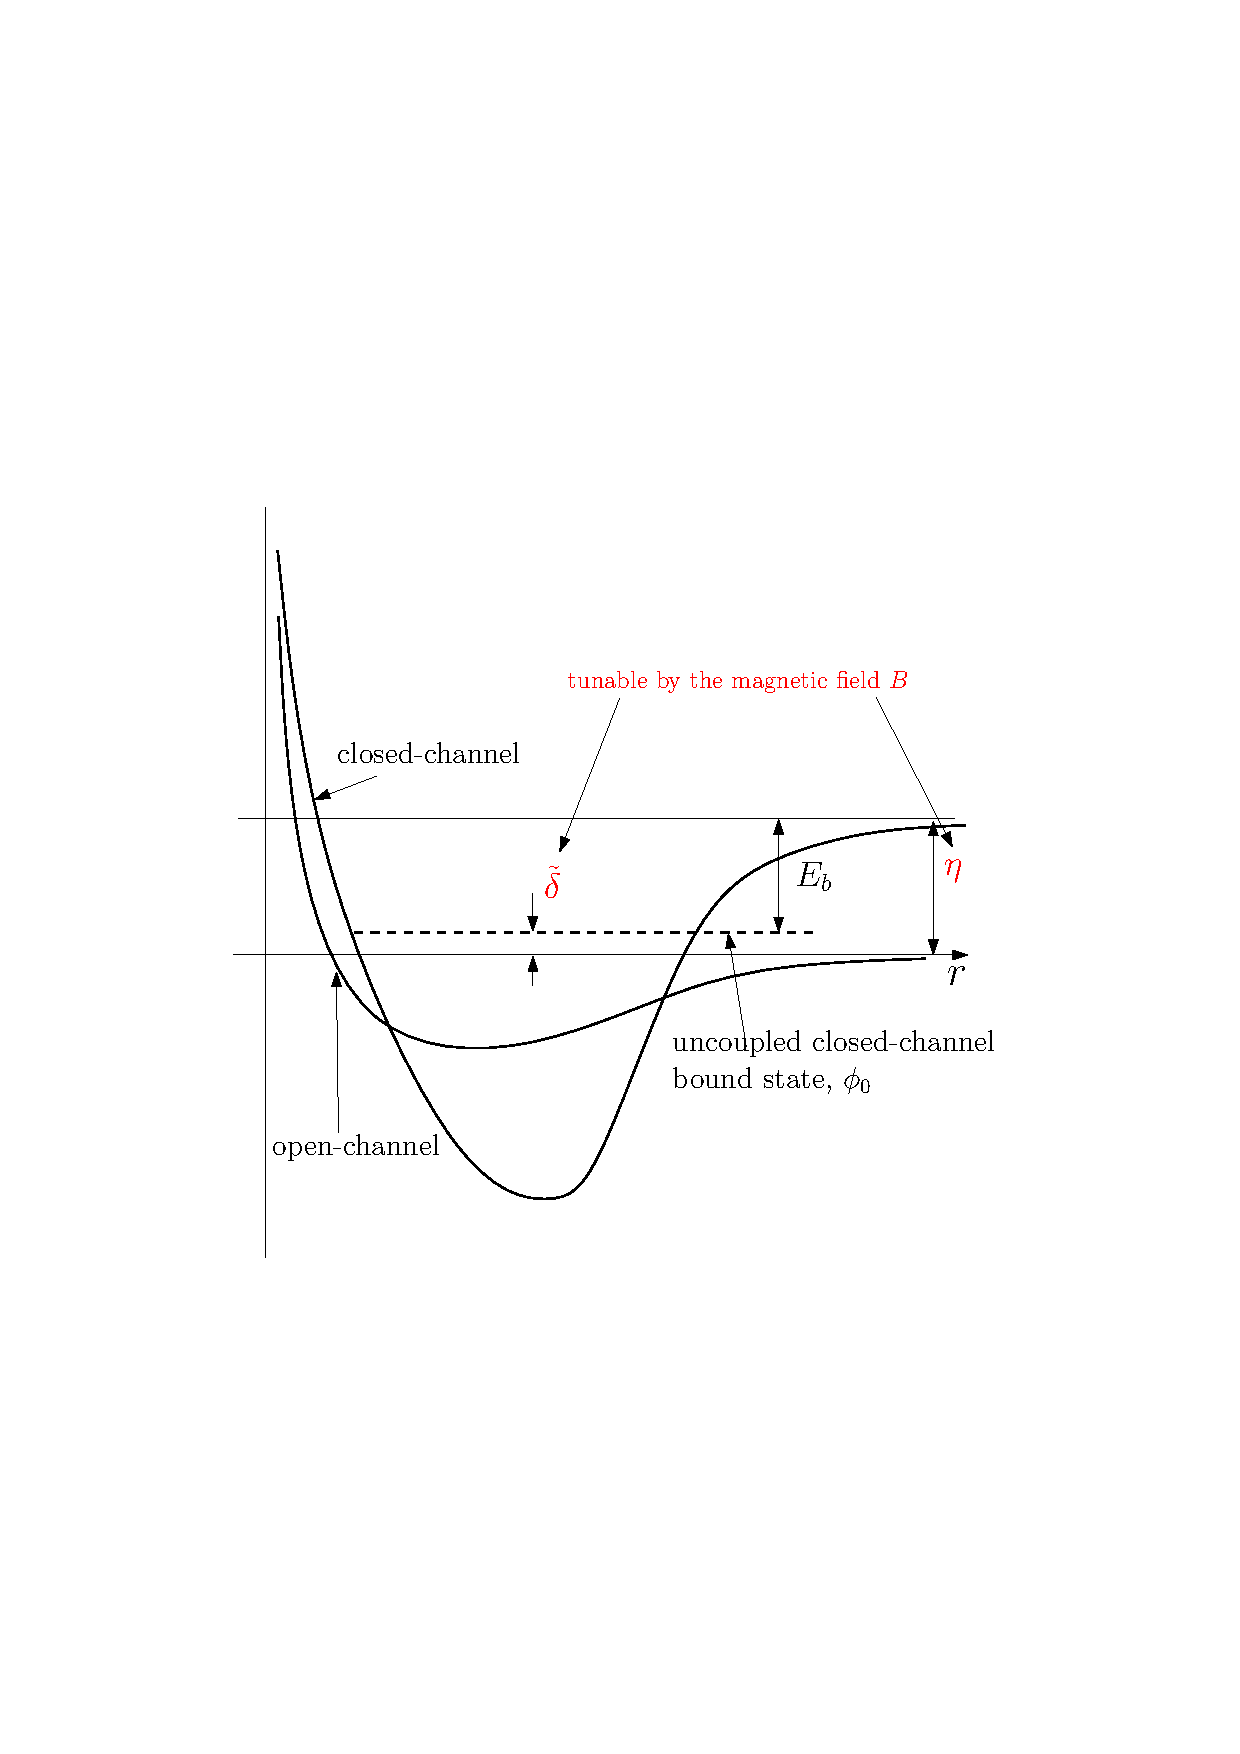
\includegraphics[width=0.8\textwidth]{2potential}

%Levels are marked with $F$ and $F_{z}$ {(see Footnote \ref{foot:intro:f} in page \pageref{foot:intro:f})} %Note that the energy of the $\ket{F=\nth{2},F_z=-\nth{2}}$ state first increases with the magnetic field, $B$, at low field then decrease at high field. In the same way, the energy of the $\ket{F=\frac{3}{2},F_z=-\nth{2}}$ state first decreases and then increases with the magnetic field.  
\label{fig:intro:li6}
\end{center}
\end{figure}
}


 \frame{
\frametitle{Scattering state and the bound state in a Feshbach resonance}
%\begin{columns}
%
%\begin{column}{0.6\textwidth}
\begin{figure}[htbp]
\begin{center}
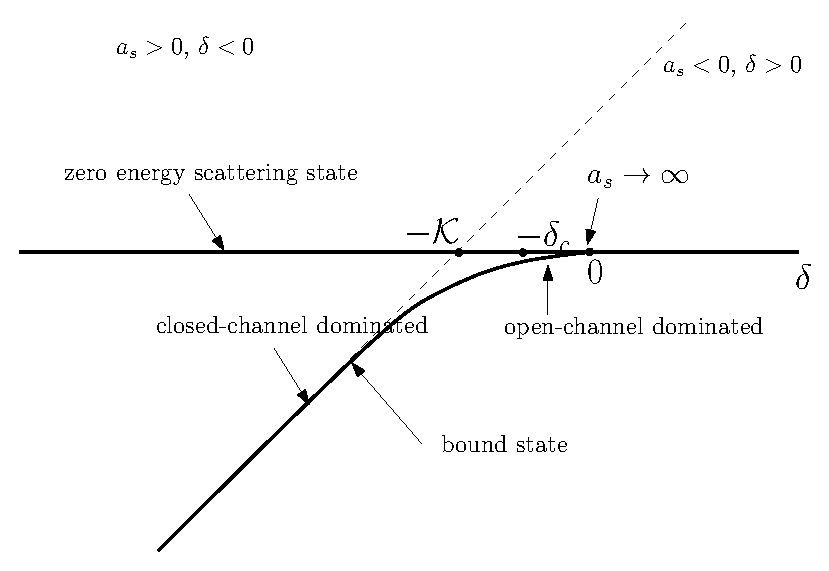
\includegraphics[width=0.6\textwidth]{levels}
%\caption{Energy levels in a Feshbach resonance\label{fig:intro:levels}} 
\end{center}
\end{figure}
Resonant point is not the level crossing point. The shift $\mathcal{K}$ is large than most energy scales.
$\delta=\tilde\delta-\mathcal{K}$
\begin{tabular}{|p{4cm}|p{4cm}|}
\hline
 $\mathemph{\abs{\delta}\ll\delta_{c}}$&$\mathemph{\abs{\delta}\gg\delta_{c}}$\\\hline
 Atoms are predominantly in the open-channel.&Atoms are predominantly in the closed-channel.\\
 \hline
\end{tabular}
%\end{column}
%\begin{column}{0.35\textwidth}

%\end{column}
%\end{columns}
}


\begin{frame}
\frametitle{Broad and narrow Feshbach resonance }

  Broad or narrow are \myemph{many-body} concepts. 
        Comparing $\delta_c$ with the many-body scale, $E_F$
 
       \myemph{Broad resonance}: $\mathemph{\delta_c\gg{}E_F}$
        \begin{itemize}

\item The closed channel weight is negligible everywhere.
\item The closed channel is just like a simple knob for $a_{s}$
\item The single-channel models' solutions are directly applied.
\end{itemize}
   

              
 
       \myemph{Narrow resonance}:  $\mathemph{\delta_c\ll{}E_F}$
        \begin{itemize}

\item The closed channel weight is substantial or even dominant close to the resonance.
\item Both channels need to be considered in the many-body framework. 
\item Studied by Gurarie and Radzihovsky \footnote{[Gurarie and Radzihovsky, Annals of Physics, 322(1):2 � 119.  2007]}
\end{itemize}
\end{frame}

\frame{
\frametitle{Three species problem}
\begin{itemize}
\item Two channels might share a common hyperfine species.
\item Interchannel Pauli exclusion between two channels.
\item No counterpart in the two-body physics.  
\item Only important in narrow resonance. 
\item Example: the resonance close to 834G in $^{6}$Li, open-channel: $\ket{\frac{1}{2},-\nth{2}}\otimes\ket{\nth{2},+\nth{2}}$; closed-channel: $\ket{\frac{3}{2},-\nth{2}}\otimes\ket{\nth{2},+\nth{2}}$

\end{itemize}
}

\section[Single-channel]{Single-channel crossover}
\frame{
\frametitle{Single-channel crossover}
\begin{itemize}
\item  $\prod_{\vk}(u_{vk}+v_{\vk}a^{\dg}_{\uparrow\vk}a^{\dg}_{\downarrow-\vk})\ket{0}=A\exp{}(\sum_{\vk}c_{\vk}a^{\dg}_{\uparrow\vk}a^{\dg}_{\downarrow-\vk})\ket{0}$
\item Continuously varying interactions ($a_{s}$)
\end{itemize}
\begin{figure}[htbp]
\begin{center}
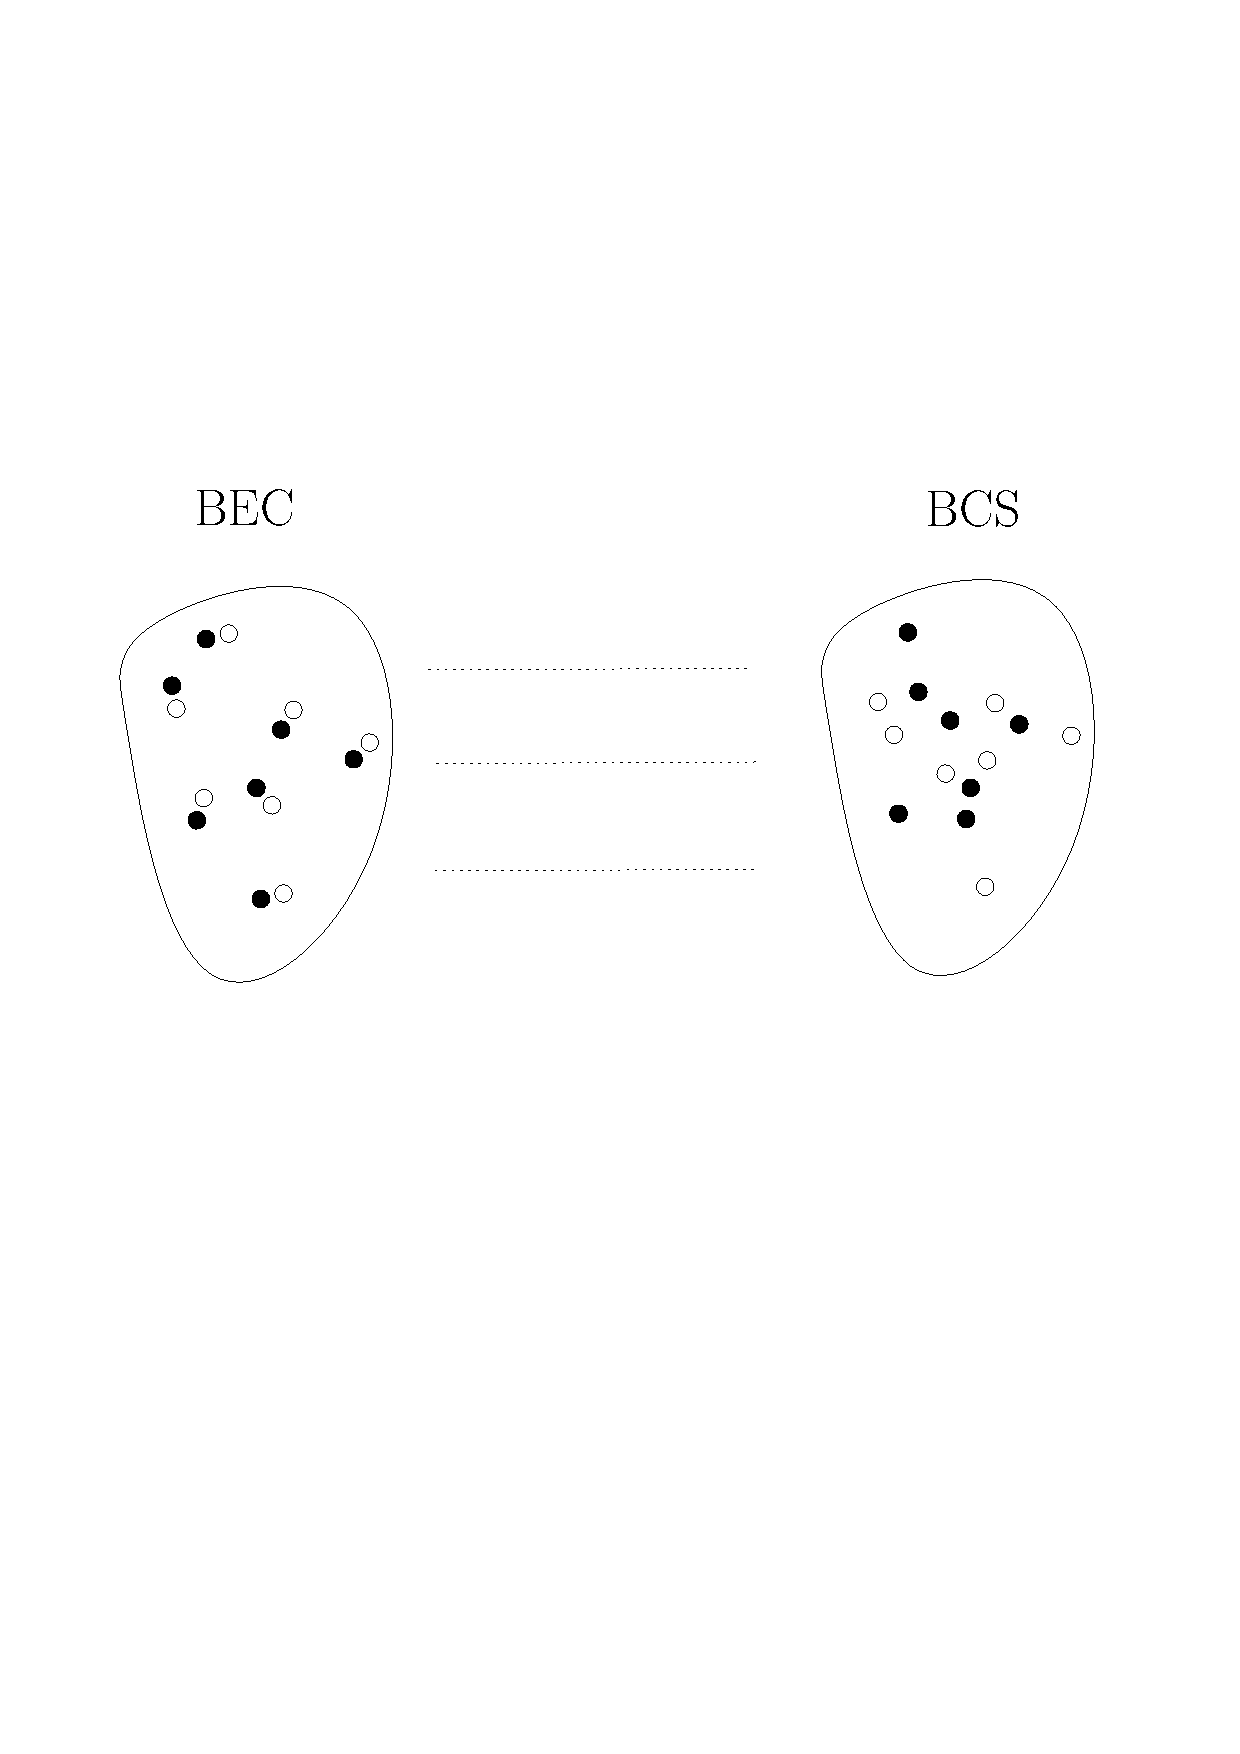
\includegraphics[width=0.7\textwidth]{crossover}
%\caption{Energy levels in a Feshbach resonance\label{fig:intro:levels}} 
\end{center}
\end{figure}
}
\frame{
\frametitle{The gap equation and the number equation}
 \myemph{The renormalized gap equation}
\begin{equation}\label{eq:pathInt:gapRenormalized}
\boxed{-\frac{m\mathcal{V}_{0}}{4\pi{}a_{s}}=\sum_{\vk}\mbr{\frac{\tanh{(E_k/2T)}}{2E_k}-\nth{2\epsilon_{\vk}}}}
\end{equation}
$E_\vp=\sqrt{\xi_\vp^2+\abs{\Delta_0}^2}$

\myemph{The number equation}
\begin{equation}
\boxed{N=\nth{L^{d}}\sum_{\vk}\mbr{1-\frac{\epsilon_{\vk}}{E_{\vk}}\tanh{(\frac{E_{\vk}}{2T})}}}
\end{equation}

}

\frame{
\frametitle{$\mu$ and $\Delta$ in the crossover}
\begin{figure}[htbp]
\begin{center}
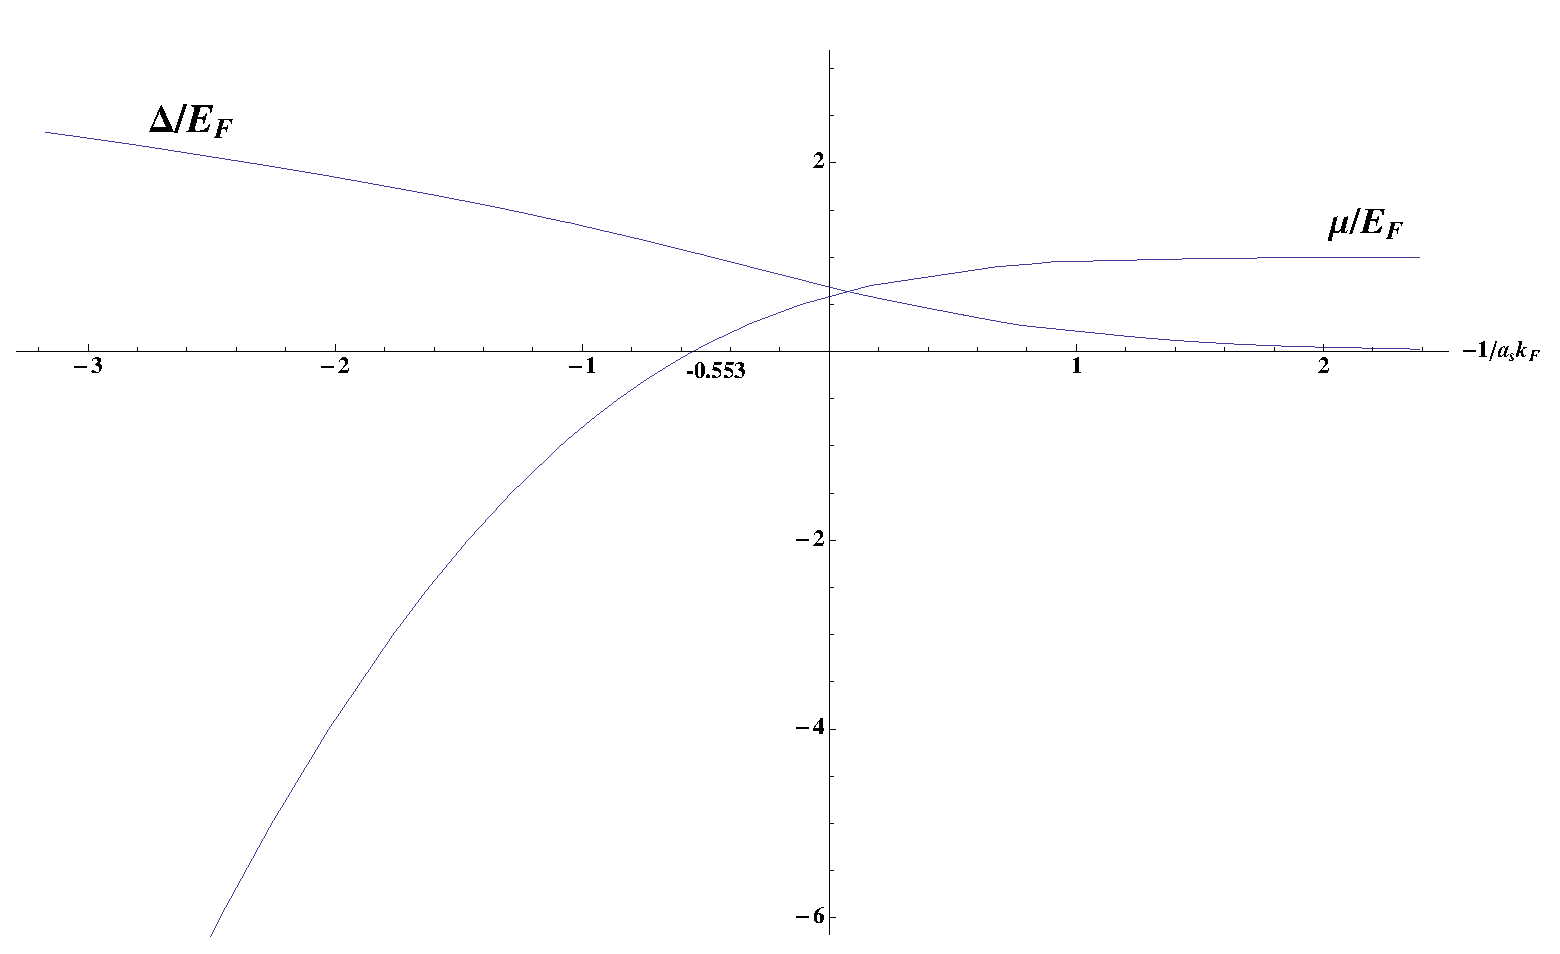
\includegraphics[width=0.8\textwidth]{SingleChannelCrossoverMuDelta}
\caption{The chemical potential $\mu$ and gap $\Delta$ in the mean field level over crossover} 
\label{fig:pathInt:meanField}
{\small All quantities in the unit of energy ($\mu$, $\Delta$) are rescaled with the Fermi energy $E_{F}$ and the s-wave scattering length $a_{s}$ is rescaled with $1/k_{F}$.  }
\end{center}
\end{figure}
}


\section[Two-channel]{Two-channel crossover model}
\frame{
\frametitle{Two-channel model}
\begin{itemize}
\item Two order parameters 
 \begin{equation}\label{eq:pathInt2:mf}
\mtrx{\Delta_1\\\Delta_2}=\mtrx{U&Y\\Y^{*}&V}\sum_{\vk}\mtrx{<{\psi_{a,-{\vk}}\psi_{b,+{\vk}}}>\\<{\psi_{a,-{\vk}}\psi_{c,+{\vk}}}>}
\end{equation}
\item Order parameters are result of mixed channel;
\item $\Delta_{1}$ corresponds to the single channel gap;
\item Reduced to the single-channel by two steps
\begin{enumerate}
\item Treat effects other than the inter-channel Pauli exclusion in a non-perturbative way;
\item Treat the inter-channel Pauli exclusion perturbavtively. 
\end{enumerate}
\end{itemize}


 

}
\frame{
\frametitle{Extremely narrow resonance}
The coupling between two channels is assumed to be extremely weak ($Y\to0$). $\mathcal{K}\to0$, $\delta_{c}\to0$. Two channels share the same chemical potentials. 
\begin{figure}[hhtb]
	\centering
	         \subfloat[$E_{F}<\tilde\delta$]{\label{fig:narrowFR:aboveSea}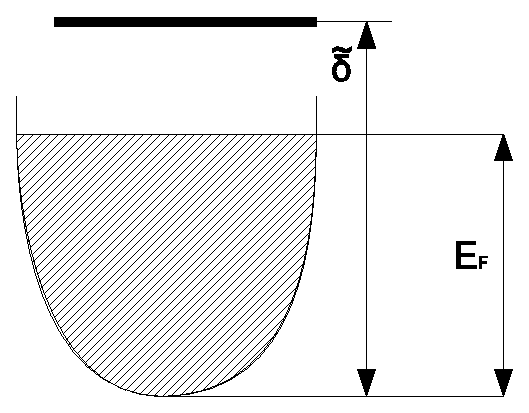
\includegraphics[width=.2\textwidth]{narrowFRabove.eps}}\quad
		\subfloat[$0<\tilde\delta<E_{F}$]{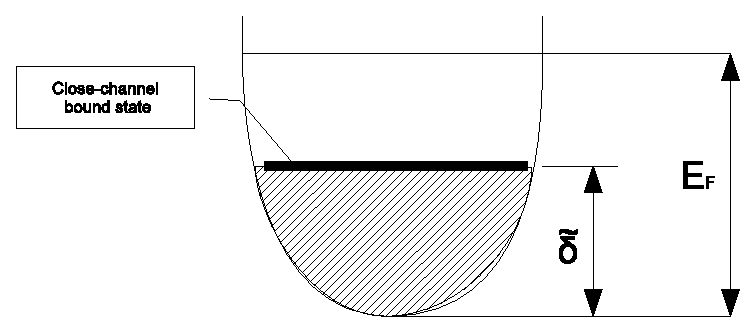
\includegraphics[width=.30\textwidth]{narrowFRin.eps}\label{fig:narrowFR:inSea}}\quad
		\subfloat[$\tilde\delta<0$]{\label{fig:narrowFR:belowSea}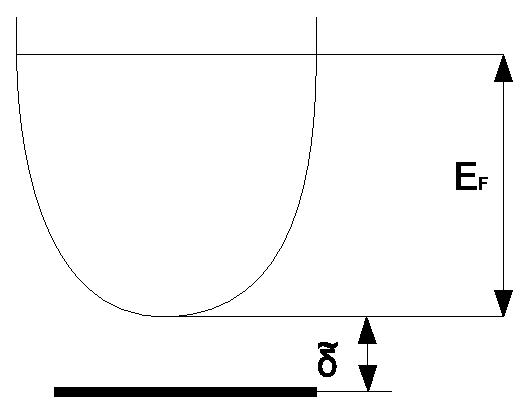
\includegraphics[width=.20\textwidth]{narrowFRbelow.eps}}
	%\caption{Extremely narrow resonance\label{fig:narrowFR}}
	%\small{The shaded area is occupied by atoms. }
	%\parbox{0.7\textwidth}{\small{  In Fig. \subref{fig:narrowFR:inSea} chemical potential would be close to the closed-channel bound state level (besides small shift due to the open-channel intra-channel coupling) and the ``Fermi sea'' above is empty. }}
\end{figure}
\begin{itemize}
\item Energy is counted from Fermi surface
\item Atoms distributed in both channels. 
\item The inter-channel Pauli exclusion persists in (b)
\end{itemize}
}

\frame{
	\frametitle{Narrow resonance w/o interchannel Pauli exclusion}
	
	\begin{itemize}
\item Energy zero moves to the Fermi surface
\begin{gather}
1=-\mbr{\frac{4\pi{\mathemph{\tilde{a}_{s}}(\mu)}}{m}\sum(\nth{2E_{\vk}}-\nth{2\epsilon_{\vk}})}\label{eq:pathInt2:narrowGapS}\\
\tilde{a}_{s}=a_{\text{bg}}(1+\frac{\mathcal{K}}{\delta-\mathemph{2\mu}})\approx{}\frac{a_{\text{bg}}\mathcal{K}}{\delta-\mathemph{2\mu}}
\end{gather}
\item Extra counting for the closed-channel. 
\begin{gather}
\mathemph{N_{\text{open}}}=\sum_\vk\frac{E_\vk-\xi_\vk}{2E_\vk}\label{eq:pathInt2:narrowNumS}
\end{gather}
\item  Studied by Gurarie and Radzihovsky \footnote{[Gurarie and Radzihovsky, Annals of Physics, 322(1):2 � 119.  2007]}
\end{itemize}
}
\frame{
\frametitle{Narrow resonance w/o interchannel Pauli exclusion}
\begin{figure}[htbp]
\begin{center}
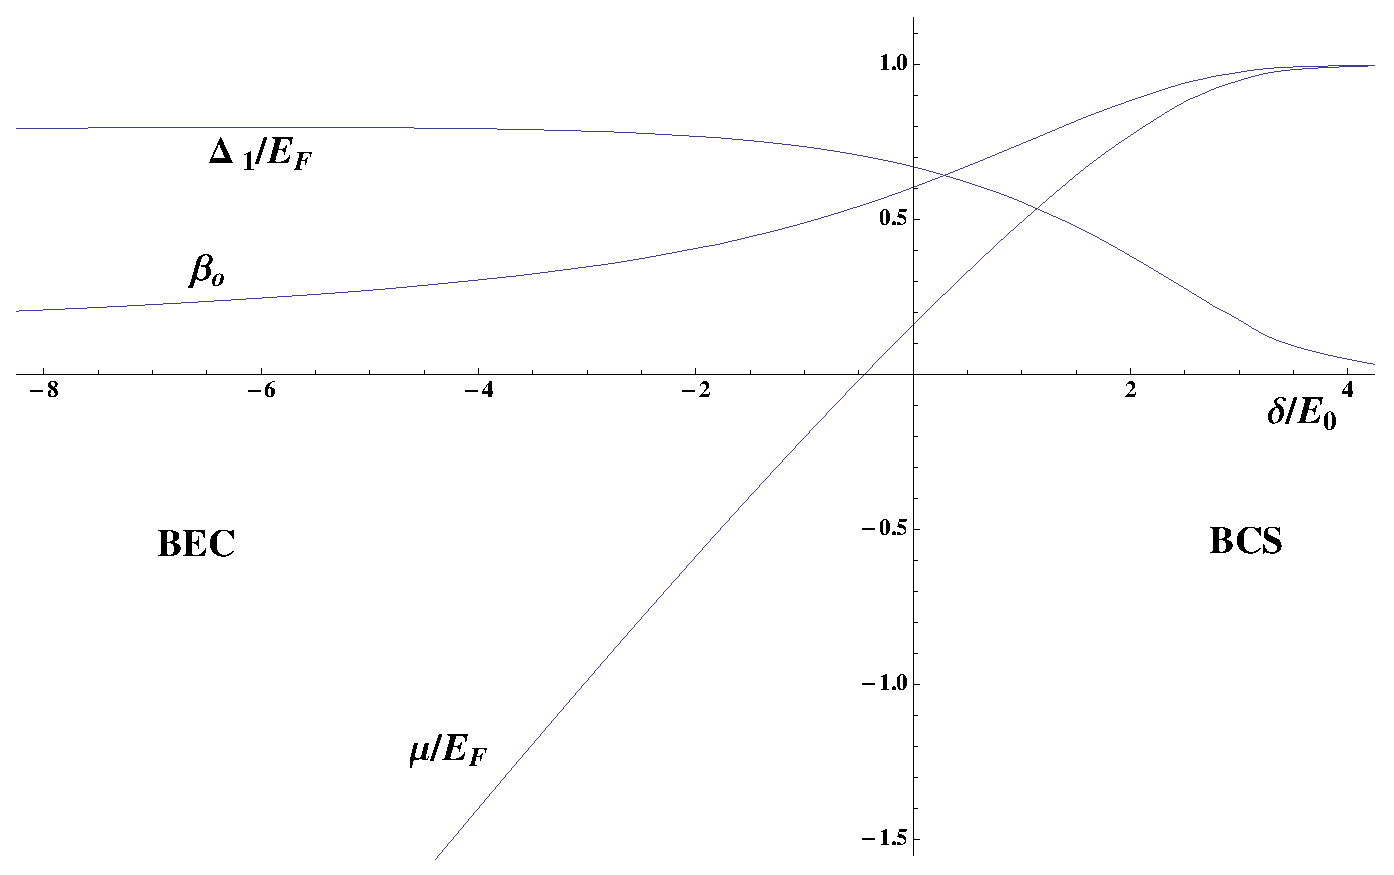
\includegraphics[width=0.8\textwidth]{narrow}
%\caption{The chemical potential $\mu$, the open-channel gap $\Delta_{1}$ and the open-channel relative weight $\beta_{o}$ over crossover with the narrow Feshbach resonance without considering the inter-channel Pauli exclusion  vs. the chemical potential and the gap in the single-channel model} 
\label{fig:pathInt2:narrow}
%{\small  The gap in the open-channel $\Delta_{1}$ and the chemical potential $\mu$ are rescaled with the the Fermi energy of the total density, $E_{F}^{(tot)}$.  The $x$-axis is the detuning $\delta$ rescaled with $E_{0}$ (see Eq. \ref{eq:pathInt2:E0}) for the narrow resonance; while it is $-1/a_{s}k_{F}$ for the single-channel curves. We have taken $\delta_{c}=0.001E_{F}^{(tot)}$ for the narrow resonance figure. We used the detuning from the resonant point  for the $x$-axis in the narrow resonance instead of $-1/a_{s}k_{F}$ in the single-channel because the additional shift, $2\mu$, considering in Eq. \ref{eq:pathInt2:simplenarrowAs}.  Consequently, the chemical potential lines in both cases cross the $x$-axis at the same point where $\mu=0$.  }
\end{center}
\end{figure}
\begin{itemize}
\item $\Delta_{1}$ saturates in BEC side
\item $\tilde{a}_{s}$ differs from two-body $a_{s}$ with special shift $2\mu$
\item $\beta_{o}=\frac{n_{open}}{n_{total}}$ deviates from 1 substantially at universality

\end{itemize}
}


\frame{
\frametitle{Interchannel Pauli exclusion}
\begin{itemize}
\item Determined by the overlap between two channels
\item One simplification: \myemph{the uncoupled closed-channel bound state, $\phi_{0}$, is much smaller than the interparticle distance in size}. 
\item Size of $\phi_{0}$ in the closed-channel: $\sim{E_{b}}^{-1/2}$
\item Size of atoms in the open-channel: interparticle distance $a_{0}\sim{}E_{F}^{-1/2}$
\item Controlling parameter
\begin{equation}\label{eq:pathInt2:zetaDef}
\boxed{\zeta=\frac{\Delta_{2}^{2}}{\Delta_{1}\eta}\sim\br{\frac{E_{F}}{E_{b}}}^{1/2}\ll1}
\end{equation}
\end{itemize}
}
\frame{
\frametitle{Fermionic modes and Bogoliubov transformation}
\begin{align*}
E_{1\vk}&\approx{}E_{\vk}+u_{\vk}^{2}\Delta_{1}\zeta\\
E_{2\vk}&\approx{}E_{\vk}-v_{\vk}^{2}\Delta_{1}\zeta\\
E_{3\vk}&\approx{}\epsilon_{\vk}+\eta+\frac{\zeta}{2}\Delta_{1}
\end{align*}
\begin{itemize}
\item $E_{1\vk}$ and $E_{2\vk}$ are like Bogoliubov quasi-paticle;
\item $E_{3\vk}$ is the free fermionic excitation in the close-channel;
\item The correction is in the order of $\zeta\ll1$;
\item The correction is due to the inter-channel Pauli exclusion and does not disappear even at the extremely narrow limit. 
\end{itemize}

}
\frame{
\frametitle{Bosonic modes}
\begin{itemize}
\item Order parameters describe the collective properties of atoms;
\item Fluctuations of the order parameters;
\item Four possible modes for two complex order parameters ($\Delta_1$, $\Delta_2$);
\item The overall phase fluctuation mode is the Goldstone mode;
\item The other three modes are massive;
\item The inter-channel out-of-sync phase mode is gapped at pair-breaking energy;
\item Corrections due to the inter-channel Pauli exclusion is in the order of $\zeta$.
\end{itemize}
}

\section{Discussion}
\frame{
\frametitle{Discussion}
\begin{itemize}
\item Handle two-channel problem, especially the inter-channel Pauli exclusion, self-consistently;
\item Inter-channel Pauli exclusion can be handled by perturbation method;
\item Methodology about narrow resonance is still valid for non-simple-BCS treatment about crossover;
\item Finite temperature: BCS $\Rightarrow$ Fermi liquid; BEC $\Rightarrow$ normal dimer gas.  
\end{itemize}
}
\end{document}

